%%
%% This is file `tikzposter-template.tex',
%% generated with the docstrip utility.
%%
%% The original source files were:
%%
%% tikzposter.dtx  (with options: `tikzposter-template.tex')
%%
%% This is a generated file.
%%
%% Copyright (C) 2014 by Pascal Richter, Elena Botoeva, Richard Barnard, and Dirk Surmann
%%
%% This file may be distributed and/or modified under the
%% conditions of the LaTeX Project Public License, either
%% version 2.0 of this license or (at your option) any later
%% version. The latest version of this license is in:
%%
%% http://www.latex-project.org/lppl.txt
%%
%% and version 2.0 or later is part of all distributions of
%% LaTeX version 2013/12/01 or later.
%%


\documentclass{tikzposter} %Options for format can be included here

\usepackage{todonotes}

\usepackage[tikz]{bclogo}
\usepackage{lipsum}
\usepackage{amsmath}

\usepackage{booktabs}
\usepackage{longtable}
\usepackage[absolute]{textpos}
\usepackage[it]{subfigure}
\usepackage{graphicx}
\usepackage{cmbright}
%\usepackage[default]{cantarell}
%\usepackage{avant}
%\usepackage[math]{iwona}
\usepackage[math]{kurier}
\usepackage[T1]{fontenc}


%% add your packages here
\usepackage{hyperref}
% for random text
\usepackage{lipsum}
\usepackage[english]{babel}
\usepackage[pangram]{blindtext}

\colorlet{backgroundcolor}{blue!10}

 % Title, Author, Institute
\title{New York City Taxi Trip Duration Prediction}
\author{Weiling Deng}
\institute{Deakin University, Australia
}
%\titlegraphic{logos/tulip-logo.eps}

%Choose Layout
\usetheme{Wave}

%\definebackgroundstyle{samplebackgroundstyle}{
%\draw[inner sep=0pt, line width=0pt, color=red, fill=backgroundcolor!30!black]
%(bottomleft) rectangle (topright);
%}
%
%\colorlet{backgroundcolor}{blue!10}

\begin{document}


\colorlet{blocktitlebgcolor}{blue!23}

 % Title block with title, author, logo, etc.
\maketitle

\begin{columns}
 % FIRST column
\column{0.5}% Width set relative to text width

%%%%%%%%%% -------------------------------------------------------------------- %%%%%%%%%%
 %\block{Main Objectives}{
%  	      	\begin{enumerate}
%  	      	\item Formalise research problem by extending \emph{outlying aspects mining}
%  	      	\item Proposed \emph{GOAM} algorithm is to solve research problem
%  	      	\item Utilise pruning strategies to reduce time complexity
%  	      	\end{enumerate}
%%  	      \end{minipage}
%}
%%%%%%%%%% -------------------------------------------------------------------- %%%%%%%%%%


%%%%%%%%%% -------------------------------------------------------------------- %%%%%%%%%%
\block{Introduction}{
  This project required to build a model that predicts the total ride duration of taxi trips in New York City. The primary dataset is one released by the NYC Taxi and Limousine Commission, which includes pickup time, geo-coordinates, number of passengers, picktime and dropoff time, and several other variables.
    
}
%%%%%%%%%% -------------------------------------------------------------------- %%%%%%%%%%


%%%%%%%%%% -------------------------------------------------------------------- %%%%%%%%%%
\block{Dataset Loading and Description}{
\begin{itemize}
    \item
    %\emph{New York City Taxi Trip Duration Prediction}
    In this section, After we read, clearn the data and check NAs, The train data which we have 1458644 Rows and 11 columns. The test data which we have 625134 Rows and 9 columns.We built the linearregression model, using distance to predict the trip duration and test.

    \item
    Data Types
    \end{itemize} 
      
    \bigskip 
      \begin{tabular}{ l | l }
        \toprule
        Attribute     &  Description          \\
        \midrule
        vendor id               & a code indicating the provider associated with the trip record\\
        pickup datetime      &  date and time when the meter was engaged  \\
        dropoff datetime     &  date and time when the meter was disengaged  \\
        pickup longitude     &  the longitude where the meter was engaged\\ 
        pickup latitude        &  the latitude where the meter was engaged\\ 
        dropoff longitude    & the longitude where the meter was disengaged\\ 
        dropoff latitude       & the latitude where the meter was disengaged\\ 
        store and fwd flag   &  Y=store and forward; N=not a store and forward trip\\
        trip duration           & duration of the trip in seconds\\
    
        \bottomrule
      \end{tabular}



}
%%%%%%%%%% -------------------------------------------------------------------- %%%%%%%%%%


%%%%%%%%%% -------------------------------------------------------------------- %%%%%%%%%%

%\note{Note with default behavior}

%\note[targetoffsetx=12cm, targetoffsety=-1cm, angle=20, rotate=25]
%{Note \\ offset and rotated}

 % First column - second block


%%%%%%%%%% -------------------------------------------------------------------- %%%%%%%%%%
\block{Data Visualization}
{
\begin{itemize}
\item
Distance characteristic analysis
\end{itemize} 
\vspace{-0.5cm} 
\begin{tikzfigure}
\centering
\selectcolormodel{rgb}
%  \missingfigure{Testing a long text string.}
\includegraphics[width=0.15\textwidth]{figures//pe7.eps}\\
%  \caption{The amount rented at different times of the day} \label{framework}
\end{tikzfigure}
        
\begin{tikzfigure}
\centering
\selectcolormodel{rgb}
%  \missingfigure{Testing a long text string.}
\includegraphics[width=0.2\textwidth]{figures//pe8.eps}\\
%  \caption{The amount rented at different times of the day} \label{framework}
\end{tikzfigure}
}
%%%%%%%%%% -------------------------------------------------------------------- %%%%%%%%%%


%%%%%%%%%% -------------------------------------------------------------------- %%%%%%%%%%
\block{Visualize Predict Result}
{
\begin{itemize}
\item
Trip Duration Visualize Predict Result
\end{itemize} 
\vspace{-1cm} 
\begin{tikzfigure}
\centering
\selectcolormodel{rgb}
%  \missingfigure{Testing a long text string.}
\includegraphics[width=0.2\textwidth]{figures//pe15.eps}\\
%  \caption{The amount rented at different times of the day} \label{framework}
\end{tikzfigure}

}
%%%%%%%%%% -------------------------------------------------------------------- %%%%%%%%%%
% SECOND column
\column{0.5}
 %Second column with first block's top edge aligned with with previous column's top.
%%%%%%%%%% -------------------------------------------------------------------- %%%%%%%%%%
\block{Data Visualization}
{
\begin{itemize}
\item
Trip Duration characteristic analysis
\end{itemize} 
\vspace{-1cm} 
\begin{tikzfigure}
\centering
\selectcolormodel{rgb}
%  \missingfigure{Testing a long text string.}
\includegraphics[width=0.2\textwidth]{figures//pe9.eps}\\
%  \caption{The amount rented at different times of the day} \label{framework}
\end{tikzfigure}

}
%%%%%%%%%% -------------------------------------------------------------------- %%%%%%%%%%
%%%%%%%%%% -------------------------------------------------------------------- %%%%%%%%%%
\block{Select features and gropby data }{
\begin{description}
\item
Select ’trip duration’ and ’distance’ as features, groupby data to train data and test
data in the train dataframe, set 0 to 150 as train data, 150 to 180 as test data,
named as train and test
\end{description}
\vspace{-0.8cm}
\begin{tikzfigure}
\centering
\selectcolormodel{rgb}
%  \missingfigure{Testing a long text string.}
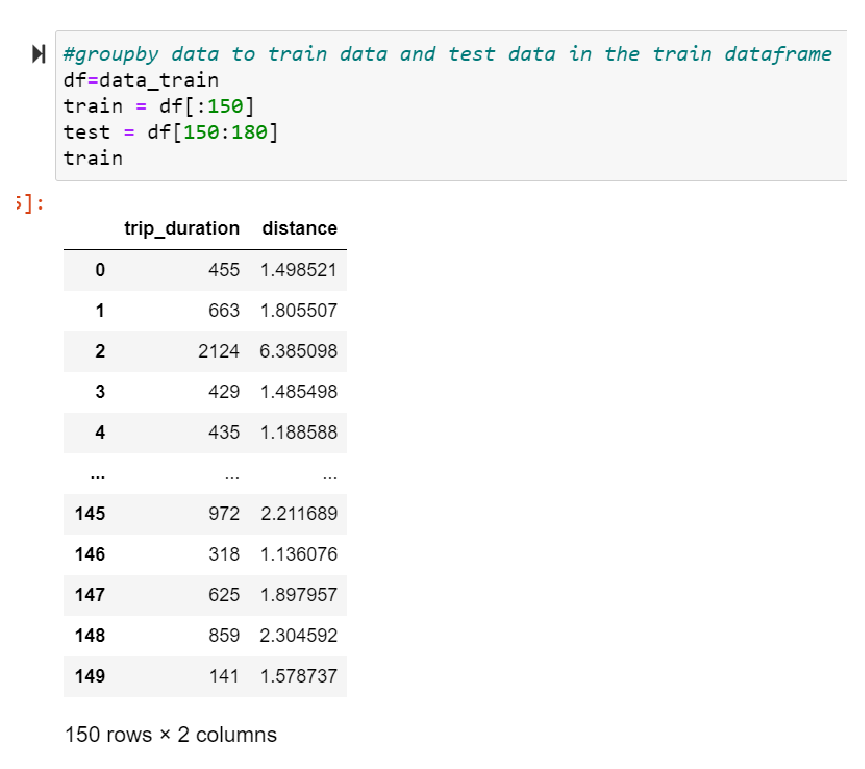
\includegraphics[width=0.4\textwidth]{figures//pe13.eps}\\
%\caption{Correlation rank} \label{framework}
\end{tikzfigure}

}
%%%%%%%%%% -------------------------------------------------------------------- %%%%%%%%%%
% Second column - first block


%%%%%%%%%% -------------------------------------------------------------------- %%%%%%%%%%
\block[titleleft]{Built Modeling and Predict Result}
{
\begin{description}
  	\item[Model:] LinearRegression Model
    
\end{description}
\vspace{.5cm}
\begin{description}
  	\item[RSMLE:] 4.616529350404572
    
\end{description}

}
%%%%%%%%%% -------------------------------------------------------------------- %%%%%%%%%%


% Second column - second block
%%%%%%%%%% -------------------------------------------------------------------- %%%%%%%%%%
\block[titlewidthscale=1, bodywidthscale=1]
{Conclusion}
{
\begin{description}
\item
  The Propose of this project which is to find the data features, select the attruibuates to built the linearregression model, find the best parameter using distance data to predict the trip duration and test.But , from the chart we can see the model is not very good, maybe we an explore other model to improve the accuracy.
\end{description}
}
%%%%%%%%%% -------------------------------------------------------------------- %%%%%%%%%%


% Bottomblock
%%%%%%%%%% -------------------------------------------------------------------- %%%%%%%%%%


%\note[targetoffsetx=8cm, targetoffsety=-10cm,rotate=0,angle=180,radius=8cm,width=.46\textwidth,innersep=.1cm]{
%Acknowledgement
%}

%\block[titlewidthscale=0.9, bodywidthscale=0.9]
%{Acknowledgement}{
%}
%%%%%%%%%% -------------------------------------------------------------------- %%%%%%%%%%

\end{columns}


%%%%%%%%%% -------------------------------------------------------------------- %%%%%%%%%%
%[titleleft, titleoffsetx=2em, titleoffsety=1em, bodyoffsetx=2em,%
%roundedcorners=10, linewidth=0mm, titlewidthscale=0.7,%
%bodywidthscale=0.9, titlecenter]

%\colorlet{noteframecolor}{blue!20}
\colorlet{notebgcolor}{blue!20}
\colorlet{notefrcolor}{blue!20}
\note[targetoffsetx=-13cm, targetoffsety=-12cm,rotate=0,angle=180,radius=8cm,width=.96\textwidth,innersep=.4cm]
{
\begin{minipage}{0.3\linewidth}
\centering

\includegraphics[width=24cm]{logos/tulip-wordmark.eps}
\end{minipage}
\begin{minipage}{0.7\linewidth}
{ \centering
 The $11^{th}$ International Conference on Knowledge Science,
  Engineering and Management (KSEM 2018),
  17-19/08/2018, Changchun, China
}
\end{minipage}
}
%%%%%%%%%% -------------------------------------------------------------------- %%%%%%%%%%


\end{document}

%\endinput
%%
%% End of file `tikzposter-template.tex'.
